\documentclass[11pt]{article}

\usepackage[T1]{fontenc}
\usepackage[utf8]{inputenc}
\usepackage[a4paper,margin=0.8in]{geometry}
\usepackage{graphicx}
\usepackage{amsmath,amssymb}
\usepackage{booktabs}
\usepackage{array}
\usepackage{hyperref}
\usepackage{xcolor}
\usepackage{caption}
\usepackage{subcaption}
\usepackage{float}
\usepackage{enumitem}
\usepackage{microtype}
\usepackage{placeins}

\graphicspath{{figures/}}

\hypersetup{
    colorlinks=true,
    linkcolor=blue,
    citecolor=blue,
    urlcolor=blue
}

\title{\textbf{Phase Stability Diagnostics for Polar-Motion State-Space Analysis}\\\large A Methodological Guide to Manifold Departure, Curvature, Hysteresis, and Historical Analogue Scoring}
\author{Craig Stone}
\date{\today}

\begin{document}

\maketitle

\begin{abstract}
This paper documents the methodology and interpretation of the Phase Stability diagnostic layer used in the DRIFT polar-motion dashboard. The diagnostic framework is designed to determine whether a recent phase trajectory remains within the historically occupied \(\theta\)--\(\omega\) manifold, or whether it exhibits off-manifold motion, abnormal curvature, hysteresis, weak historical precedent, or escape-like behavior. The method is deliberately comparative rather than causal. It does not identify a physical driver by itself, nor does it assert that a core--mantle decoupling event is occurring. Instead, it provides a disciplined state-space reading of the observed trajectory relative to the historical polar-motion record. The central diagnostics are the phase-conditioned angular-velocity anomaly \(Z_{\omega}\), the phase-space curvature \(\kappa\), the normalized manifold-departure score \(M\), the hysteresis index \(H\), the historical analogue score \(A\), and the composite Coupling Stability Index \(C\). A documented 2026-05-10 example is used to show how the diagnostics are read in practice, and a four-product comparison demonstrates that the present escape-candidate classification is robust across JPL EOP2, C04/IAU2000A, finals.all/IAU2000, and finals.all/IAU1980 realizations.
\end{abstract}

\section{Purpose of the Phase Stability Layer}

The Phase Stability layer was introduced to answer a simple question: does the recent polar-motion phase trajectory behave like a normal member of the historical state-space family, or does it depart from the historical manifold in a coherent and measurable way?

The underlying phase portrait is constructed in \(\theta\)--\(\omega\) space, where \(\theta\) represents the instantaneous phase angle of the polar-motion state and \(\omega\) represents its angular velocity. Over the historical record, the system does not occupy this space uniformly. It forms a structured manifold: a narrow, recurrent, phase-conditioned corridor with loops, excursions, and preferred branches. The Phase Stability layer quantifies the relation of the recent trajectory to that historical structure.

The method is designed to distinguish three situations that can otherwise look similar by eye. First, an ordinary loop may appear visually dramatic but remain inside the historical corridor. Second, a noisy fluctuation may briefly leave the central band but lack coherent curvature or persistence. Third, a genuine state-space departure may combine large phase-conditioned velocity anomaly, abnormal curvature, poor historical analogue support, and possibly hysteresis on return. The purpose of the diagnostic is to separate these cases.

\section{Definitions}

Let the polar-motion state at time \(t\) be represented by a phase angle \(\theta(t)\) and an angular velocity \(\omega(t)\). The phase angle is usually wrapped to the interval \([-\pi,\pi]\), while the angular velocity is expressed in radians per day.

The historical record is used to estimate the expected angular velocity conditional on phase angle. For each phase bin \(\theta_i\), the historical distribution of \(\omega\) is summarized by a robust central value and robust dispersion,

\begin{equation}
\mu_{\omega|\theta_i} = \operatorname{median}\{\omega(t): \theta(t) \in \theta_i\},
\end{equation}

\begin{equation}
\sigma_{\omega|\theta_i} = 1.4826 \cdot \operatorname{MAD}\{\omega(t): \theta(t) \in \theta_i\},
\end{equation}

where MAD is the median absolute deviation. This robust construction prevents isolated historical outliers from dominating the estimated phase-conditioned envelope.

The diagnostic then asks how far the recent trajectory lies from this historical corridor.

\section{Phase-Conditioned Angular-Velocity Anomaly}

The primary local anomaly score is the phase-conditioned angular-velocity anomaly,

\begin{equation}
Z_{\omega}(t) = \frac{\omega(t)-\mu_{\omega|\theta(t)}}{\sigma_{\omega|\theta(t)}}.
\end{equation}

This quantity measures whether the system is moving unusually fast or unusually slow for its present phase angle. It is not a global anomaly score. It is local to the phase state. A value of \(\omega\) that is ordinary at one phase angle may be abnormal at another.

The absolute value \(|Z_{\omega}|\) is usually used for severity classification:

\begin{table}[H]
\centering
\caption{Interpretation of the phase-conditioned angular-velocity anomaly.}
\begin{tabular}{>{\raggedleft\arraybackslash}p{0.22\linewidth} p{0.62\linewidth}}
\toprule
\(\boldsymbol{|Z_{\omega}|}\) & Interpretation \\
\midrule
\(0\)--\(1.0\) & Ordinary; close to the historical phase-conditioned corridor. \\
\(1.0\)--\(1.5\) & Mildly displaced, usually not meaningful by itself. \\
\(1.5\)--\(2.5\) & Watch range; the state is noticeably displaced. \\
\(2.5\)--\(3.5\) & Excursion range; the state is materially off the ordinary corridor. \\
\(>3.5\) & Strong escape-candidate behavior, subject to confirmation by other diagnostics. \\
\bottomrule
\end{tabular}
\end{table}

A favorable value is therefore a small value of \(|Z_{\omega}|\). An unfavorable value is a large value of \(|Z_{\omega}|\), especially when it persists or coincides with high curvature.

\section{Historical Phase Envelope}

The historical phase envelope is the graphical companion to \(Z_{\omega}\). It is constructed by plotting the robust median \(\mu_{\omega|\theta}\) and its confidence bands,

\begin{equation}
\mu_{\omega|\theta} \pm n\sigma_{\omega|\theta},
\end{equation}

where \(n\) is typically 1, 2, or 3. The envelope allows the recent trajectory to be read directly against the historically occupied phase-conditioned manifold.

A favorable trajectory remains close to the median corridor or within the ordinary envelope. An unfavorable trajectory leaves the envelope coherently, particularly if it forms a new branch, plunging lobe, or return path displaced from the outbound path.

\section{Curvature Diagnostic}

A trajectory can be off-manifold without being dynamically interesting if it is merely displaced by noise. Curvature helps determine whether the trajectory is reorganizing in phase space.

The phase-space curvature is computed as

\begin{equation}
\kappa(t) =
\frac{\left|\dot{\theta}(t)\ddot{\omega}(t)-\dot{\omega}(t)\ddot{\theta}(t)\right|}
{\left(\dot{\theta}(t)^2+\dot{\omega}(t)^2\right)^{3/2}}.
\end{equation}

In practice, \(\theta\) and \(\omega\) should be lightly smoothed before derivatives are computed, and angular wrapping must be handled before finite differences are taken.

Low curvature means the trajectory is proceeding along a smooth or familiar branch. High curvature means the trajectory is bending sharply, possibly indicating recapture, branch transition, or altered phase relation. Curvature is most informative when it rises before or during a manifold departure.

\section{Manifold Departure Score}

The normalized manifold-departure score \(M(t)\) converts \(|Z_{\omega}|\) into a bounded diagnostic. A simple and effective first implementation is

\begin{equation}
M(t) = \min\left(\frac{|Z_{\omega}(t)|}{Z_{\mathrm{crit}}},1\right),
\end{equation}

where \(Z_{\mathrm{crit}}\) is commonly set near 3.5.

The resulting score lies between 0 and 1:

\begin{table}[H]
\centering
\caption{Interpretation of the normalized manifold-departure score.}
\begin{tabular}{>{\raggedleft\arraybackslash}p{0.22\linewidth} p{0.62\linewidth}}
\toprule
\(\boldsymbol{M}\) & Interpretation \\
\midrule
\(0.00\)--\(0.25\) & Inside or close to the historical phase manifold. \\
\(0.25\)--\(0.50\) & Mild displacement. \\
\(0.50\)--\(0.75\) & Significant excursion. \\
\(0.75\)--\(1.00\) & Strong off-manifold behavior. \\
\bottomrule
\end{tabular}
\end{table}

A favorable value is low. An unfavorable value is high. A high value does not identify a cause, but it does establish that the current state is geometrically unusual relative to the historical \(\theta\)--\(\omega\) manifold.

\section{Hysteresis Index}

A system can leave a manifold and return along the same path, or it can return along a different branch. The second case is more important because it suggests memory, path dependence, or a temporary change in the effective phase relation.

The hysteresis index compares outbound and inbound angular velocities within the same phase bins:

\begin{equation}
H(\theta_i) =
\frac{\left|\operatorname{median}(\omega_{\mathrm{out}}|\theta_i)-
\operatorname{median}(\omega_{\mathrm{in}}|\theta_i)\right|}
{\sigma_{\omega|\theta_i}}.
\end{equation}

The window-level hysteresis index may be computed as the median or maximum of valid \(H(\theta_i)\) values,

\begin{equation}
H = \operatorname{median}_{i}\,H(\theta_i).
\end{equation}

A favorable hysteresis reading is low. This means the return path overlaps the outbound path. An unfavorable hysteresis reading is high. This means the same phase sector is crossed with materially different angular velocity on the outward and return legs.

If the recent trajectory has not yet produced enough return geometry, hysteresis should be reported as unavailable rather than forced. In such cases the correct interpretation is not ``low hysteresis,'' but ``insufficient return path.''

\section{Historical Analogue Score}

The historical analogue score asks whether the recent trajectory resembles any prior historical window. It is intended to prevent overinterpretation of a visually striking but historically common structure.

For a recent trajectory segment \(R\), candidate historical windows \(W_i\) are extracted with comparable duration or sample count. The paths are normalized and compared using either a dynamic time-warping distance, a Fréchet-like path distance, or a resampled Euclidean trajectory distance. The distance \(d_i\) is then converted to a similarity score,

\begin{equation}
A_i = \exp\left(-\frac{d_i}{s}\right),
\end{equation}

where \(s\) is a scale parameter. The best historical analogue score is

\begin{equation}
A = \max_i A_i.
\end{equation}

The interpretation is inverted relative to the other severity scores: high analogue similarity is favorable because it means the current behavior has precedent.

\begin{table}[H]
\centering
\caption{Interpretation of the historical analogue score.}
\begin{tabular}{>{\raggedleft\arraybackslash}p{0.22\linewidth} p{0.62\linewidth}}
\toprule
\(\boldsymbol{A}\) & Interpretation \\
\midrule
\(>0.75\) & Strong historical analogue; behavior is comparatively ordinary. \\
\(0.50\)--\(0.75\) & Partial historical analogue; similar but not strongly matched. \\
\(0.30\)--\(0.50\) & Weak analogue; historically unusual. \\
\(<0.30\) & Poor analogue; the recent trajectory is historically novel or poorly classified. \\
\bottomrule
\end{tabular}
\end{table}

A favorable value is therefore high. An unfavorable value is low.

\section{Coupling Stability Index}

The Coupling Stability Index \(C\) is a composite state-space diagnostic. It combines several independent readings into one bounded score. A representative formulation is

\begin{equation}
C =
w_Z |Z_{\omega}|_{\mathrm{norm}}
+
w_{\kappa}\hat{\kappa}
+
w_M M
+
w_H H_{\mathrm{norm}}
+
w_A(1-A),
\end{equation}

where \(\hat{\kappa}\) is normalized curvature, \(H_{\mathrm{norm}}\) is normalized hysteresis, and \(1-A\) represents historical novelty. If hysteresis is unavailable, the remaining weights are renormalized.

A typical weighting scheme is

\begin{equation}
w_Z=0.30,\quad
w_{\kappa}=0.20,\quad
w_M=0.25,\quad
w_H=0.10,\quad
w_A=0.15.
\end{equation}

The score is read as follows:

\begin{table}[H]
\centering
\caption{Interpretation of the Coupling Stability Index.}
\begin{tabular}{>{\raggedleft\arraybackslash}p{0.22\linewidth} p{0.62\linewidth}}
\toprule
\(\boldsymbol{C}\) & Interpretation \\
\midrule
\(0.00\)--\(0.25\) & Stable; the recent trajectory remains close to the historical manifold. \\
\(0.25\)--\(0.50\) & Watch; mild to moderate instability or displacement. \\
\(0.50\)--\(0.75\) & Excursion; coherent departure or abnormal geometry. \\
\(0.75\)--\(1.00\) & Escape candidate; strong off-manifold behavior, high curvature, novelty, or combined instability. \\
\bottomrule
\end{tabular}
\end{table}

The term ``Coupling Stability Index'' should be understood as a descriptive state-space label. It does not prove a change in physical core--mantle coupling. Rather, it measures whether the observed phase relation is behaving as though the effective state-space constraint has weakened, shifted, or become temporarily nonstandard.

\section{Favorable and Unfavorable Diagnostic Regimes}

The diagnostics are most useful when read together. No single score should be treated as decisive. A favorable state has small phase-conditioned anomaly, low curvature, low manifold departure, high historical analogue similarity, low hysteresis if measurable, and a low composite index:

\begin{equation}
|Z_{\omega}| < 1.5,\quad
M < 0.25,\quad
A > 0.75,\quad
C < 0.25.
\end{equation}

An unfavorable state has elevated anomaly, high curvature, strong manifold departure, weak historical analogue support, possible hysteresis, and a high composite index:

\begin{equation}
|Z_{\omega}| > 2.5,\quad
M > 0.75,\quad
A < 0.50,\quad
C > 0.75.
\end{equation}

The most important unfavorable pattern is not a single high value, but a coherent cluster: off-manifold motion, sharp curvature, weak historical precedent, and a return path that does not retrace the outbound path.

\section{Updated 2026-05-10 Example and Cross-Product Robustness}

Figure~\ref{fig:phase-stability-four-products} shows the Phase Stability panel for the 2026-05-10 endpoint across four Earth orientation product realizations. The products differ in source and reference convention: JPL EOP2, EOP 20u24 C04 under IAU2000A, finals.all under IAU2000, and finals.all under IAU1980. The absolute values vary modestly, as expected, but the qualitative classification is invariant: all four runs classify the present state as an escape candidate.

\begin{figure}[H]
\centering
\begin{subfigure}[t]{0.4\linewidth}
\centering
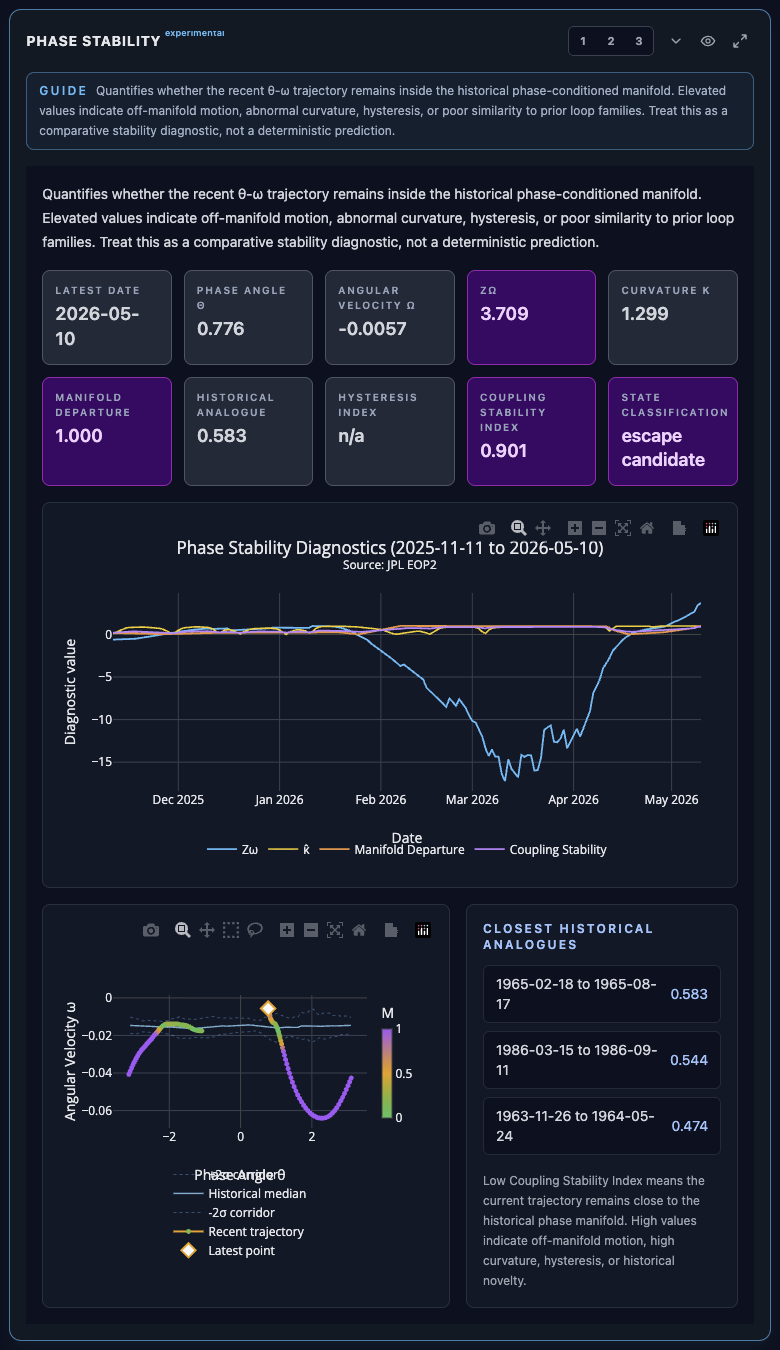
\includegraphics[width=\linewidth]{phase_stability_jpl_eop2.png}
\caption{JPL EOP2.}
\end{subfigure}\hfill
\begin{subfigure}[t]{0.4\linewidth}
\centering
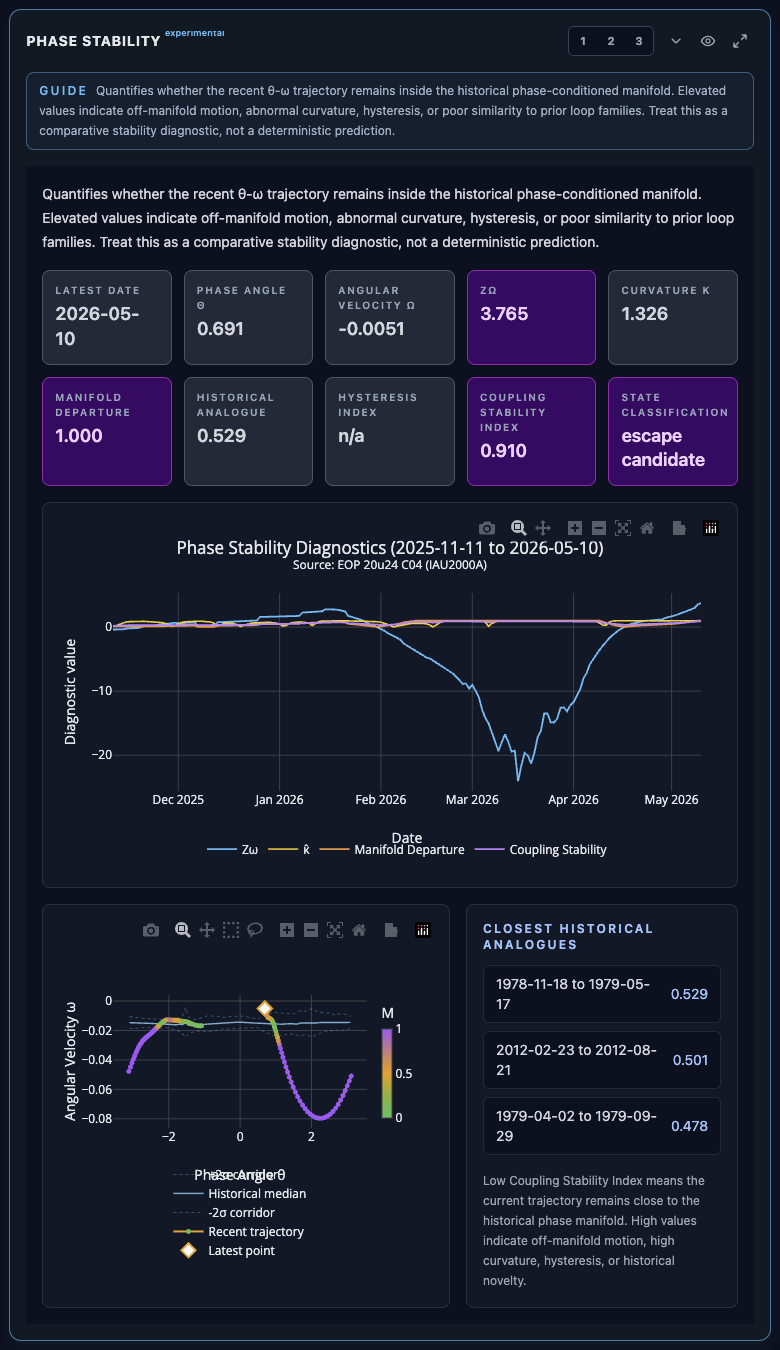
\includegraphics[width=\linewidth]{phase_stability_c04_iau2000a.png}
\caption{EOP 20u24 C04 / IAU2000A.}
\end{subfigure}

\vspace{0.6em}

\begin{subfigure}[t]{0.4\linewidth}
\centering
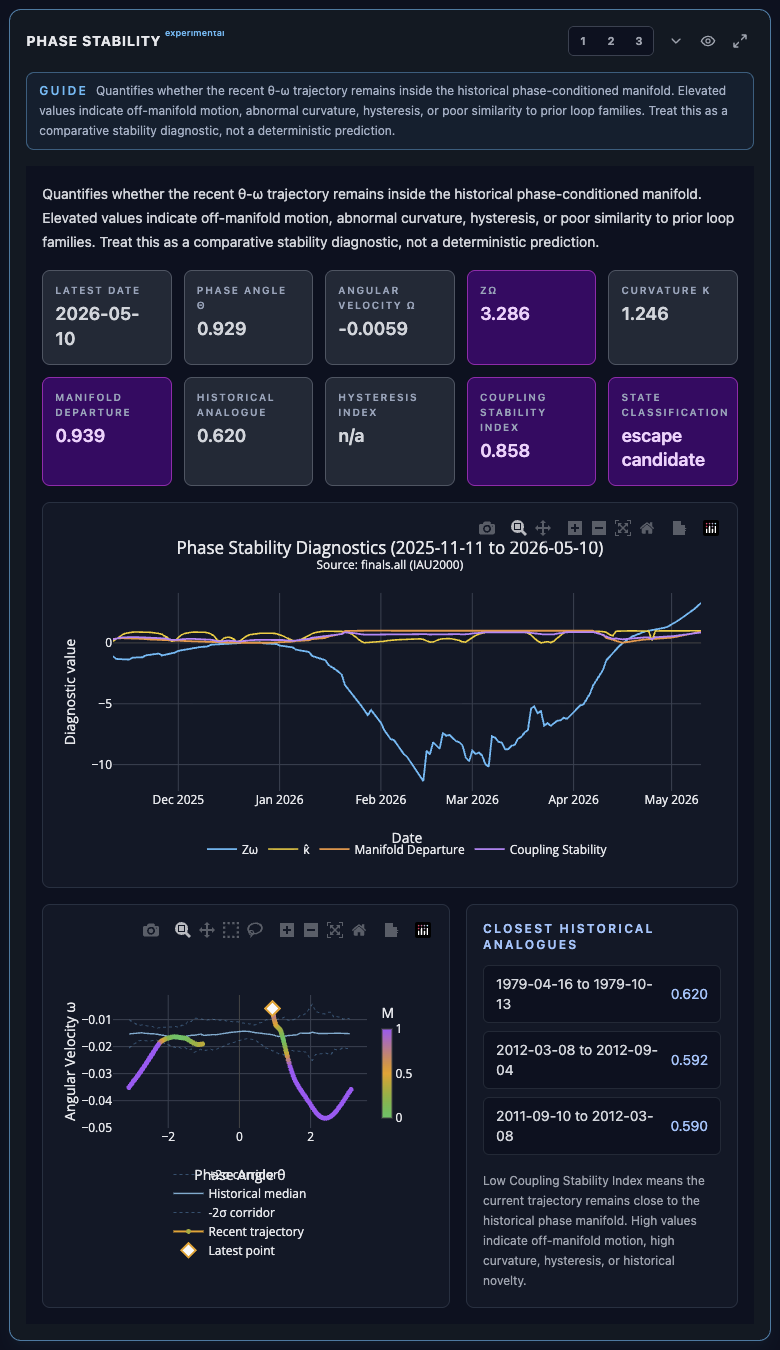
\includegraphics[width=\linewidth]{phase_stability_finals_iau2000.png}
\caption{finals.all / IAU2000.}
\end{subfigure}\hfill
\begin{subfigure}[t]{0.4\linewidth}
\centering
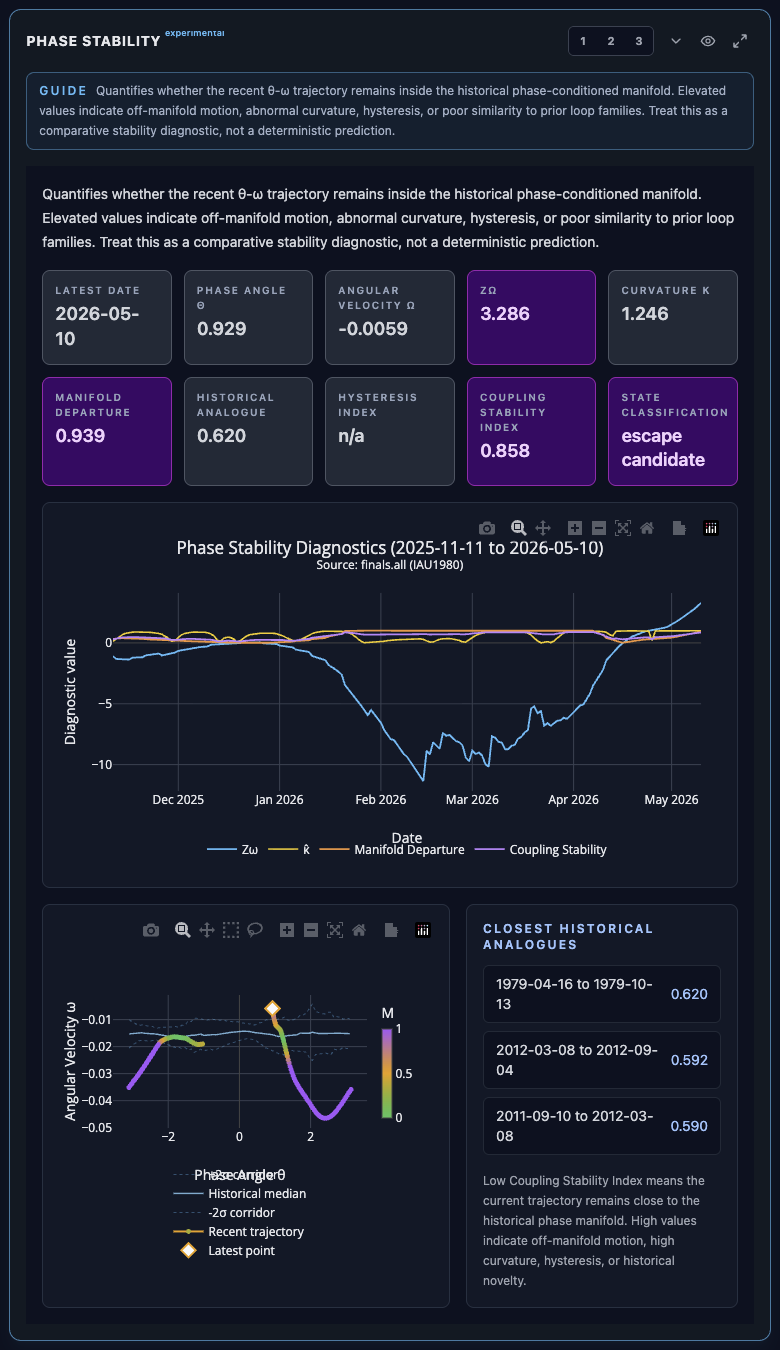
\includegraphics[width=\linewidth]{phase_stability_finals_iau1980.png}
\caption{finals.all / IAU1980.}
\end{subfigure}
\caption{Phase Stability diagnostics for the 2026-05-10 endpoint across four EOP realizations. All four products classify the recent \(\theta\)--\(\omega\) trajectory as an escape-candidate state. The numerical diagnostics vary modestly by product, but the state classification is invariant. This reduces the likelihood that the result is an artifact of a single EOP product, reference convention, or preprocessing path.}
\label{fig:phase-stability-four-products}
\end{figure}

The cross-product values are summarized in Table~\ref{tab:cross-product-summary}. Relative to the 2026-05-09 snapshot, the 2026-05-10 update strengthens the result in the C04/IAU2000A and JPL EOP2 products. Both reach the upper bound of the normalized manifold-departure score, while all four products remain in the escape-candidate regime. The finals.all IAU2000 and IAU1980 realizations remain effectively identical at this scale.

\begin{table}[H]
\centering
\caption{Cross-product Phase Stability summary for the 2026-05-10 endpoint.}
\label{tab:cross-product-summary}
\begin{tabular}{lccccccc}
\toprule
Product & \(\theta\) & \(\omega\) & \(Z_{\omega}\) & \(\kappa\) & \(M\) & \(A\) & \(C\) \\
\midrule
JPL EOP2 & 0.776 & -0.0057 & 3.709 & 1.299 & 1.000 & 0.583 & 0.901 \\
EOP 20u24 C04 / IAU2000A & 0.691 & -0.0051 & 3.765 & 1.326 & 1.000 & 0.529 & 0.910 \\
finals.all / IAU2000 & 0.929 & -0.0059 & 3.286 & 1.246 & 0.939 & 0.620 & 0.858 \\
finals.all / IAU1980 & 0.929 & -0.0059 & 3.286 & 1.246 & 0.939 & 0.620 & 0.858 \\
\bottomrule
\end{tabular}
\end{table}

The strongest reading in the updated example is the cross-product persistence of the manifold-departure signal. In the C04/IAU2000A and JPL EOP2 runs, \(M=1.000\), indicating that the recent trajectory has reached the upper bound of the normalized off-manifold score under the adopted thresholding. The finals.all realizations are slightly softer but still severe, with \(M=0.939\). The phase-conditioned anomaly remains large in all products, with \(Z_{\omega}\) ranging from 3.286 to 3.765. Curvature remains elevated, ranging from 1.246 to 1.326, which indicates that the current trajectory is not merely displaced from the historical band but is also bending sharply through phase space.

The historical analogue score moderates the interpretation. Across the four runs it ranges from 0.529 to 0.620. The episode is therefore not without precedent. It has historical cousins, including windows near 1965, 1978--1979, 1986, and 2011--2012, but it does not have a strong twin. This is the desired discipline of the method: the present episode is neither dissolved into ordinary noise nor declared unprecedented.

The unavailable hysteresis reading remains important. It means the trajectory has not yet provided enough return-path information to determine whether the system is retracing its outbound route or returning along a displaced branch. If a later return path produces high hysteresis, the case for a branch-transition interpretation would become stronger. If hysteresis remains low and the path collapses back into the historical corridor, the episode would be better interpreted as a large but bounded excursion.

\section{Geometric Context of the 2026 Phase-Stability Episode}

The Phase Stability diagnostic is not intended to stand alone. It should be read against the broader geometry of the polar-motion record. Figures~\ref{fig:phase-portrait-envelope}--\ref{fig:residual-phase-space} provide the companion views used by DRIFT: the \(\theta\)--\(\omega\) portrait, the orthogonal deviation ratio, the full polar-motion trajectory, and the residual phase-space structure.

\begin{figure}[H]
\centering
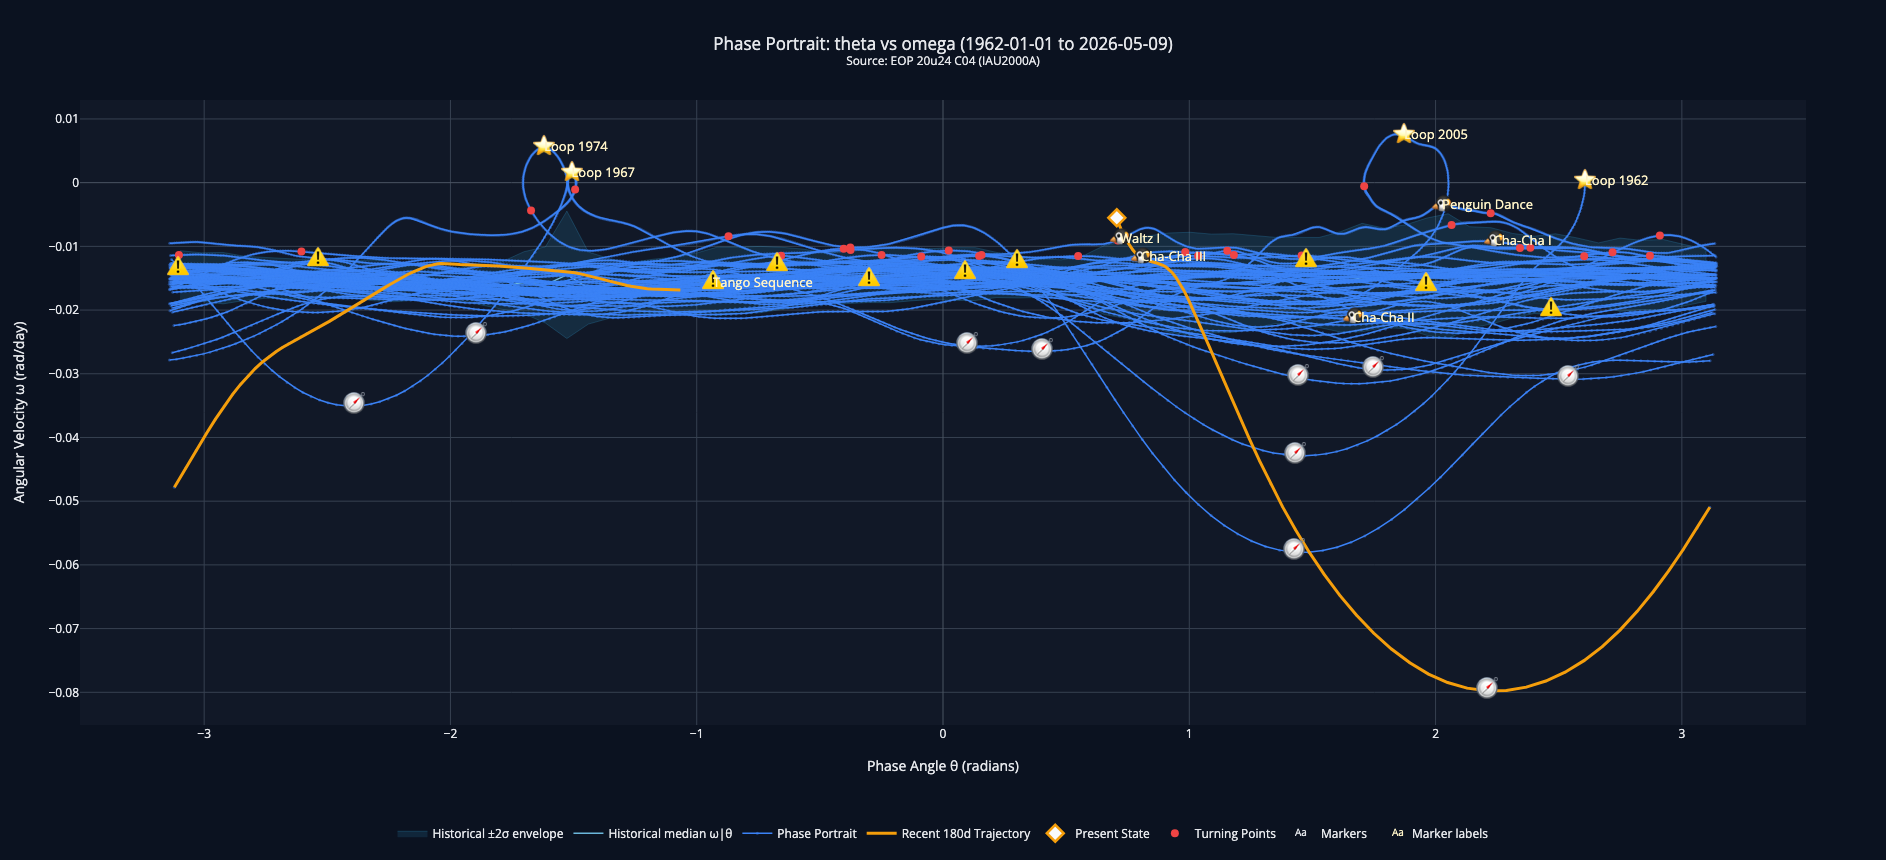
\includegraphics[width=0.98\linewidth]{phase_portrait_envelope.png}
\caption{Phase portrait of \(\theta\) versus \(\omega\), showing the historical phase-space manifold, the historical median and \(\pm 2\sigma\) corridor, the recent 180-day trajectory, the present state, turning points, and named loop structures. The recent trajectory leaves the main historical angular-velocity corridor and forms a large downward lobe before curving back toward the ordinary band. The diagnostic question is not whether the angular velocity is large in isolation, but whether it is unusual for the present phase angle.}
\label{fig:phase-portrait-envelope}
\end{figure}

\begin{figure}[H]
\centering
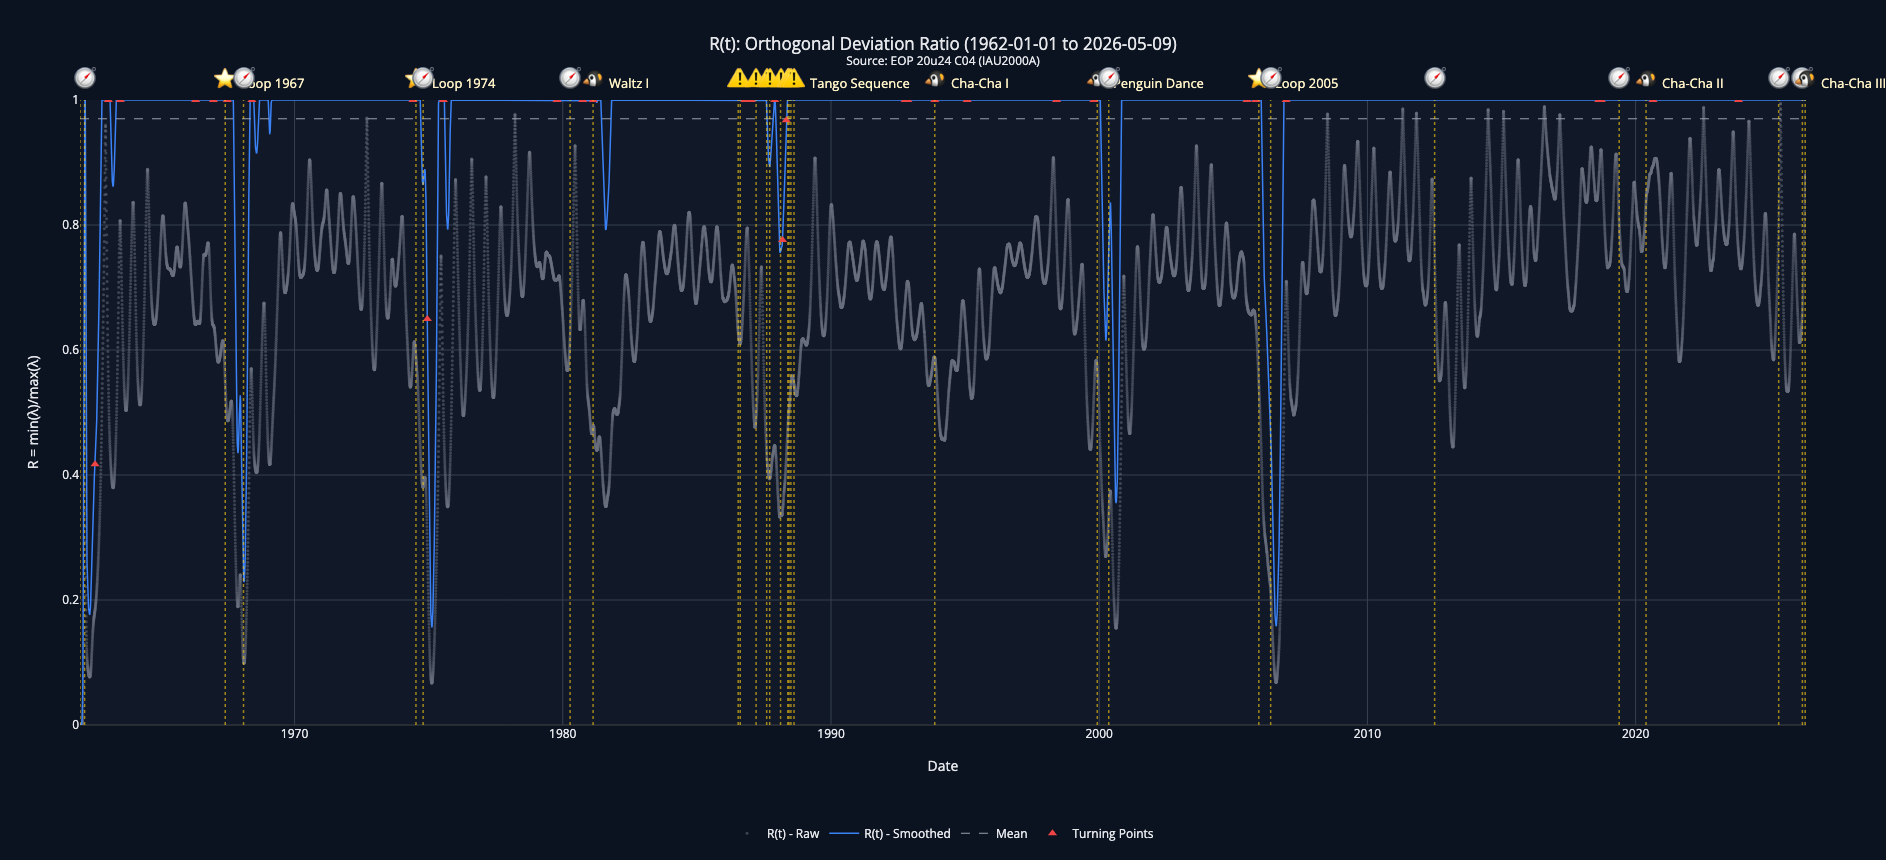
\includegraphics[width=0.98\linewidth]{orthogonal_deviation_ratio.png}
\caption{Orthogonal deviation ratio \(R(t)\), defined as the ratio of minor to major local variance components. Low values indicate broadening or weakening of local directional constraint; higher values indicate stronger elongation and local organization. Named loop episodes and turning-point markers show recurrent intervals of geometrical reorganization. This plot provides a time-domain companion to the phase portrait by showing when the local polar-motion geometry sharpens, relaxes, or reorganizes.}
\label{fig:orthogonal-deviation-ratio}
\end{figure}

\begin{figure}[H]
\centering
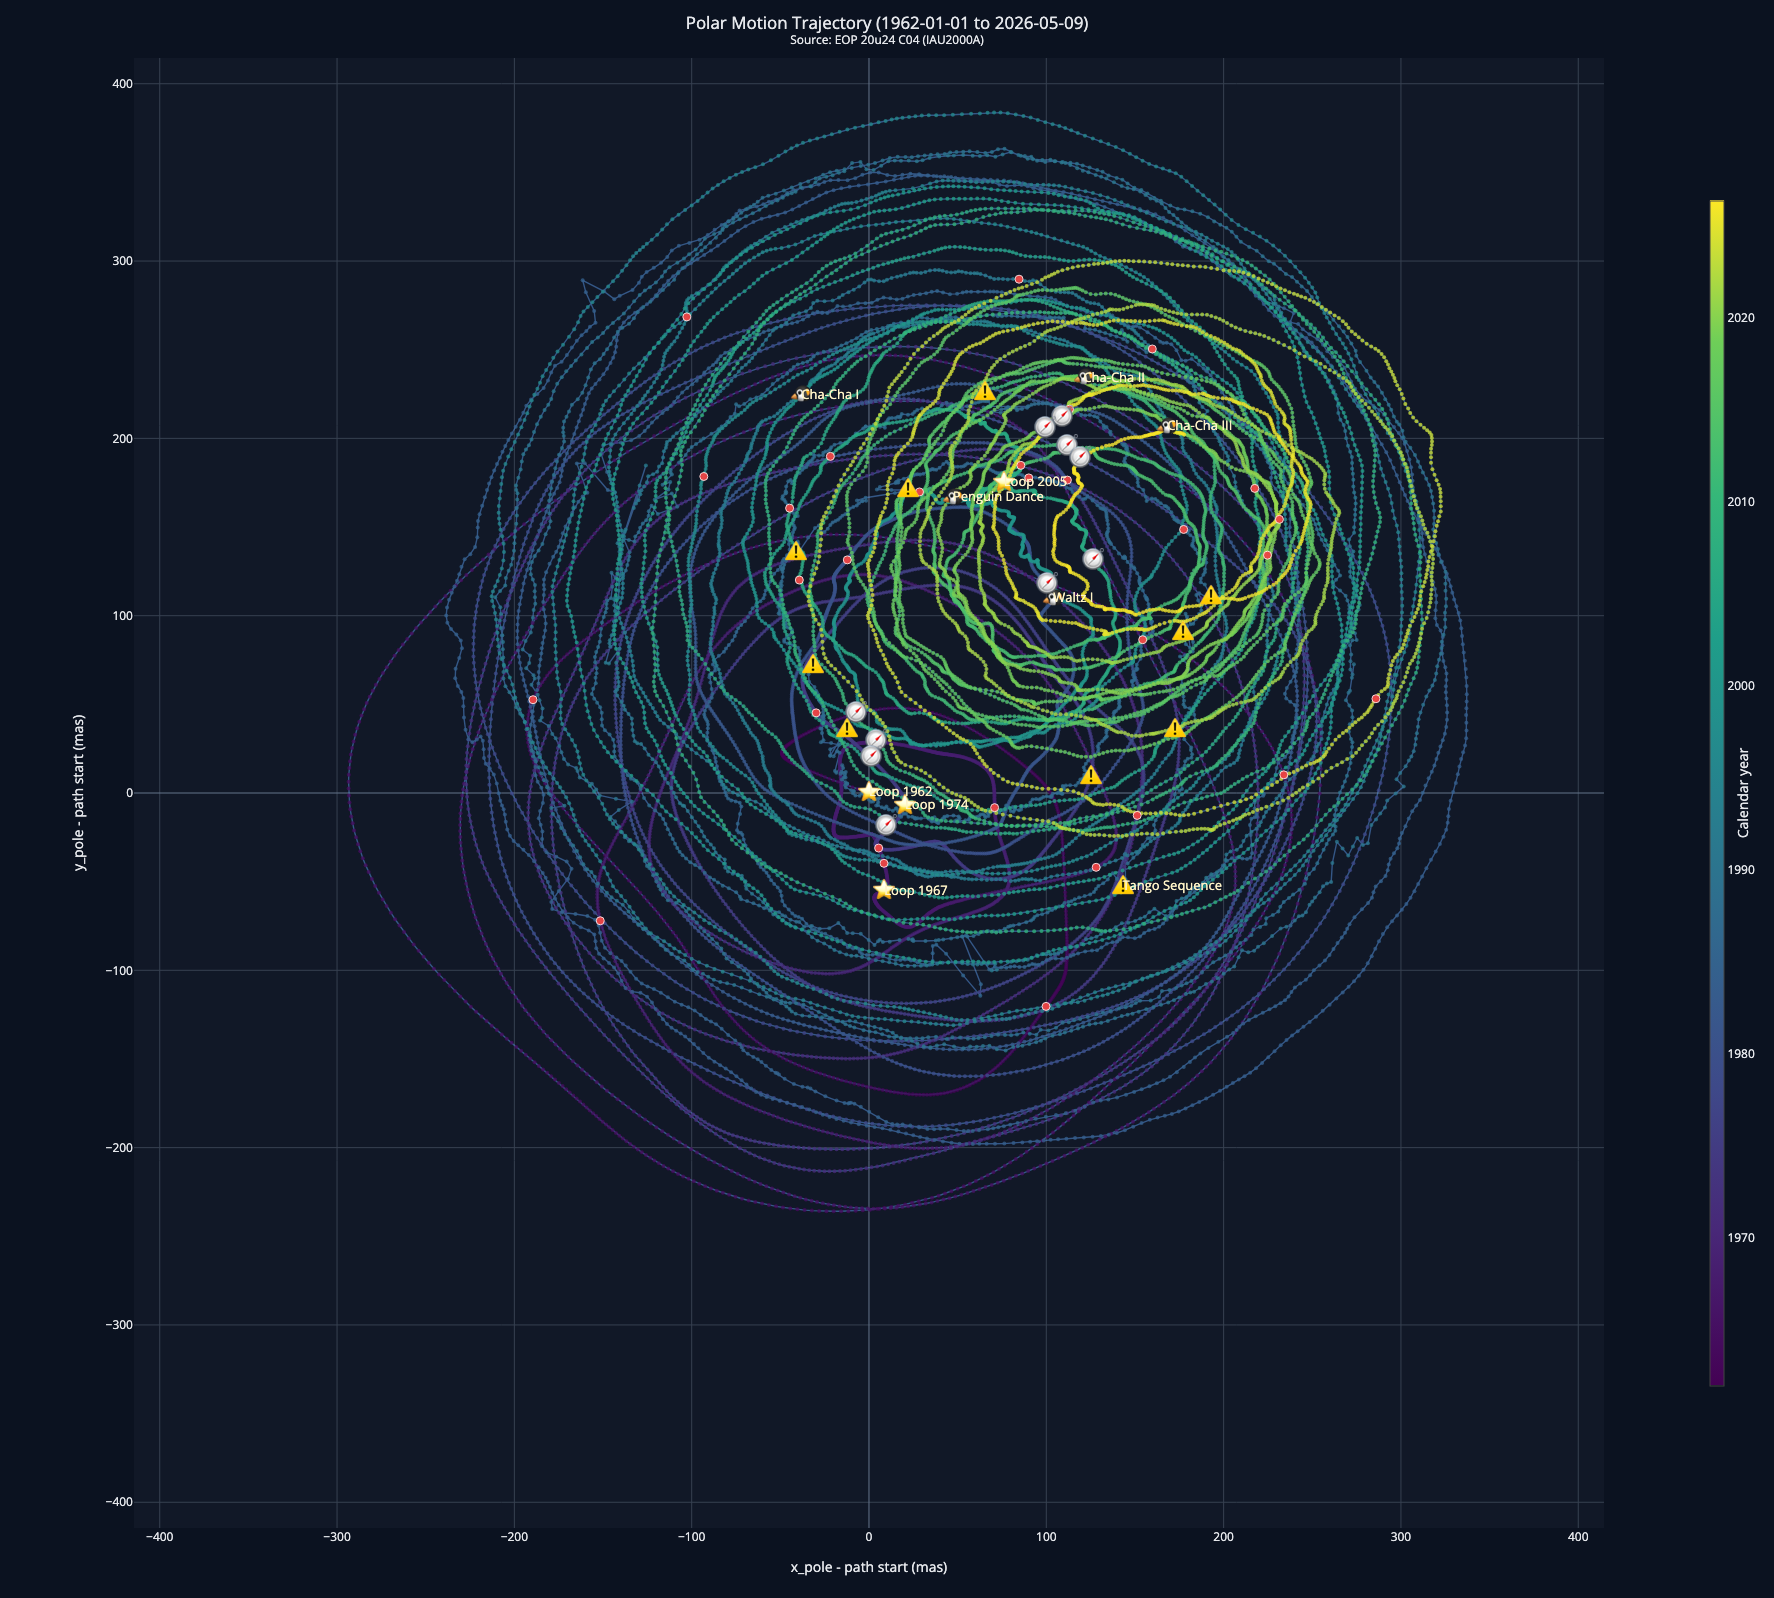
\includegraphics[width=0.86\linewidth]{polar_motion_trajectory.png}
\caption{Full polar-motion trajectory from 1962-01-01 to 2026-05-09 in path-start coordinates. The path does not fill a disk uniformly. It forms nested and migrating loop families, with labeled structures identifying recurrent episodes. The Phase Stability layer does not ask whether the pole is moving; it asks whether the current motion remains compatible with this established geometrical family.}
\label{fig:polar-motion-trajectory}
\end{figure}

\begin{figure}[H]
\centering
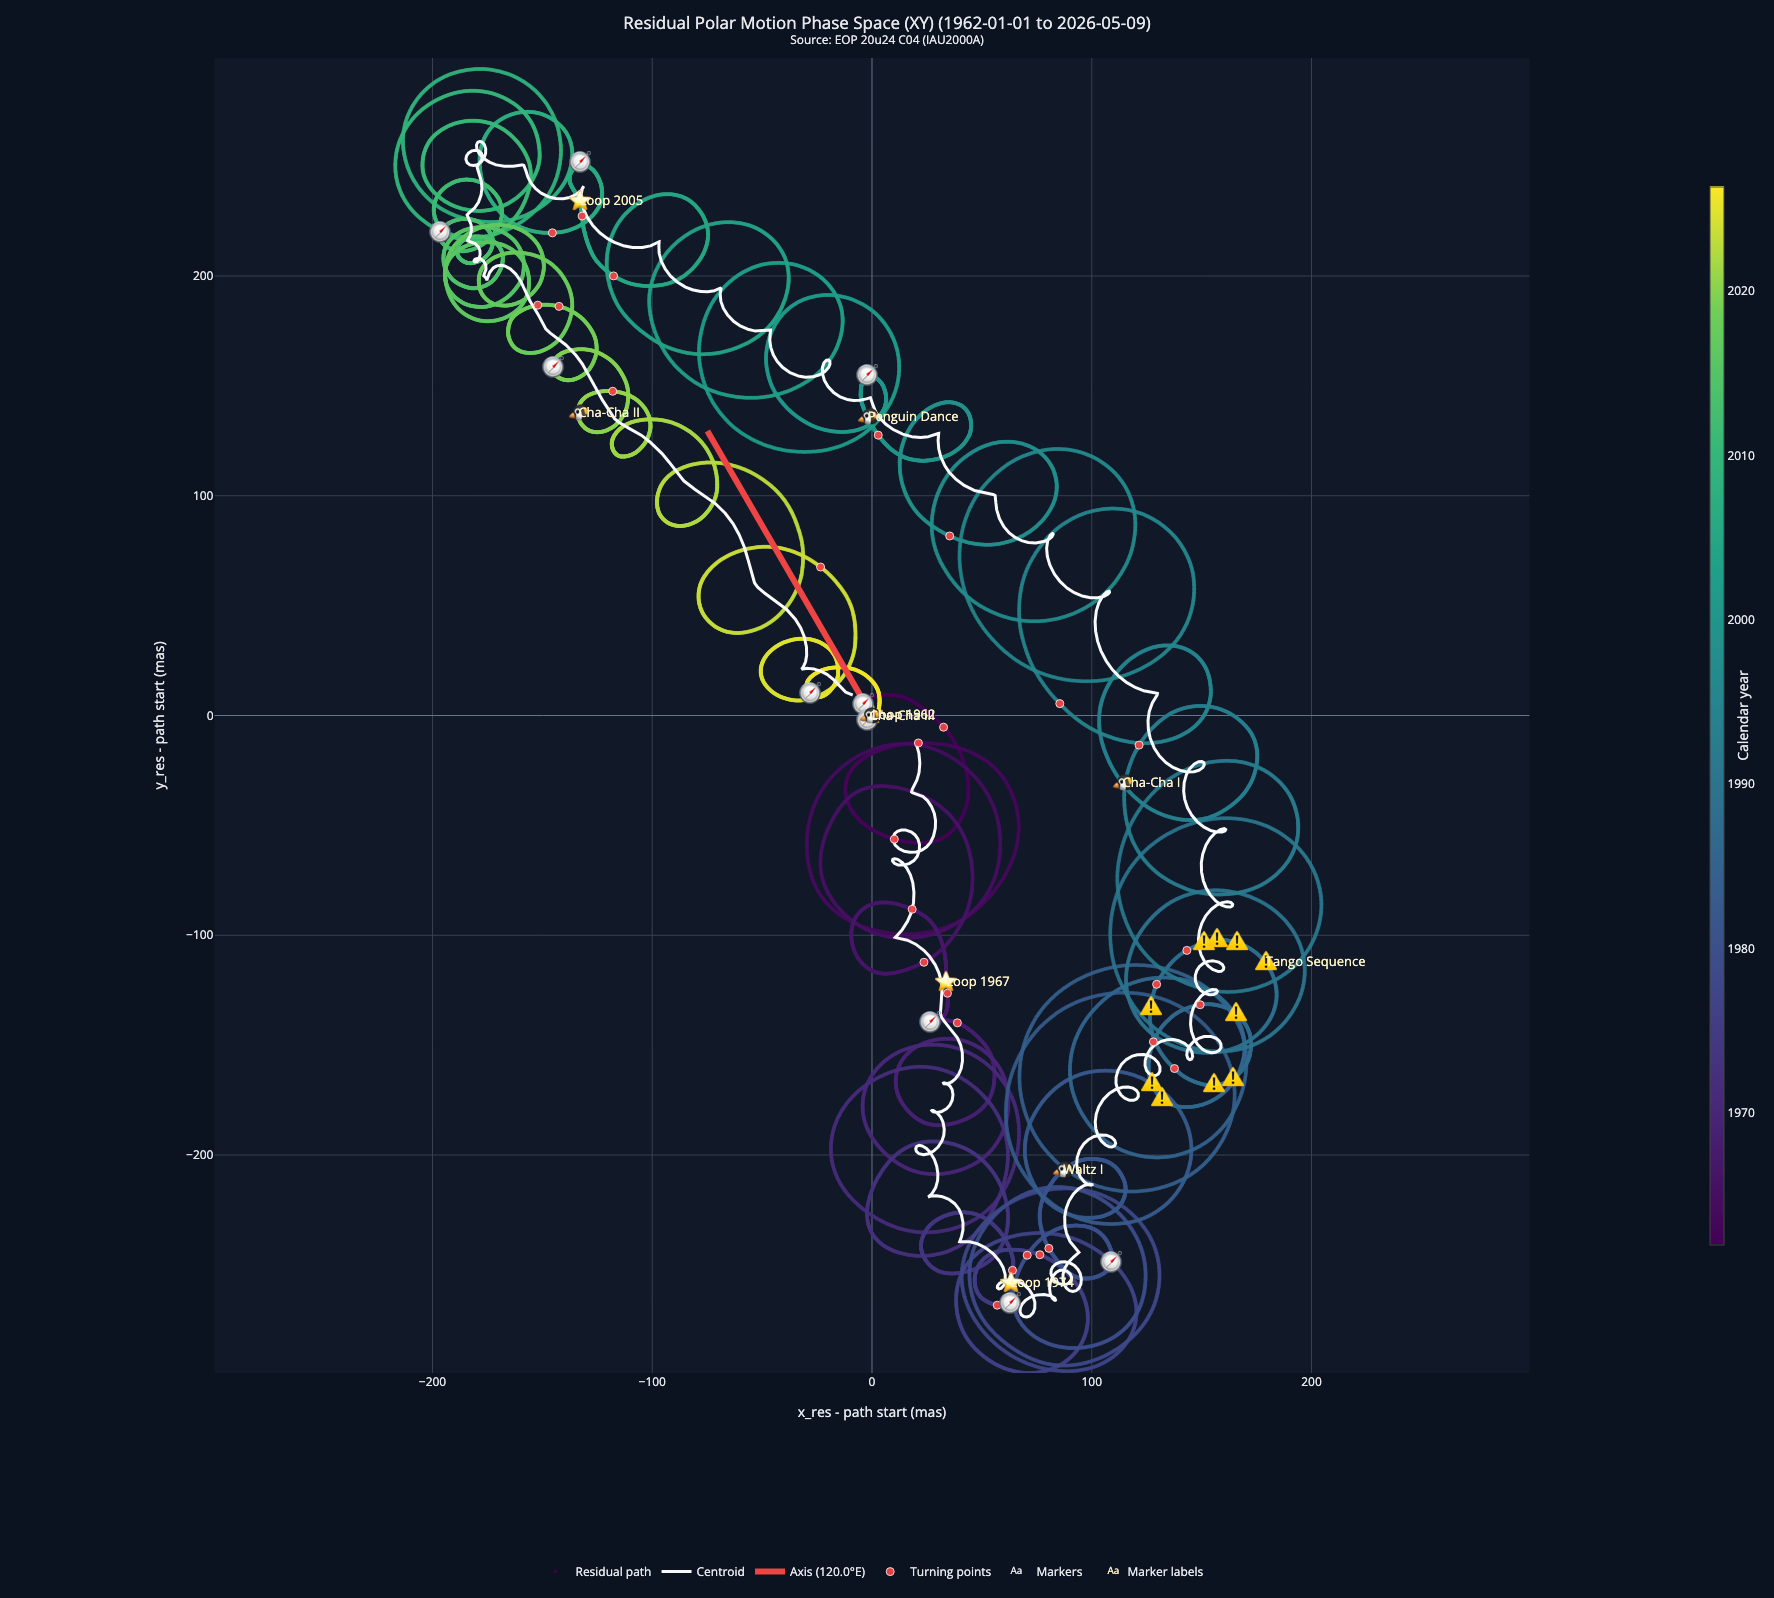
\includegraphics[width=0.86\linewidth]{residual_polar_motion_phase_space.png}
\caption{Residual polar-motion phase space after removal of the broader drift component. The residual path, centroid trace, preferred axis, and loop structures expose the organized residual component of the motion. This view is important because the present phase-stability episode is not occurring against a featureless background. It is occurring within a constrained residual geometry that has evolved coherently across the record.}
\label{fig:residual-phase-space}
\end{figure}

\FloatBarrier

\section{Reading the Updated Example in Plain Terms}

The 2026-05-10 example is unfavorable in the diagnostic sense. It does not show a quiet, historically ordinary state. It shows a recent trajectory that has moved far from the historical phase-conditioned corridor, curved strongly, and only partially resembles previous historical windows. The correct conclusion is therefore:

\begin{quote}
The recent phase trajectory is quantitatively off-manifold and presently lies in an escape-candidate state-space regime. This is a high-interest diagnostic episode requiring continued monitoring, especially for return-path hysteresis and recapture into the historical corridor.
\end{quote}

The incorrect conclusion would be:

\begin{quote}
A core--mantle decoupling event has been confirmed.
\end{quote}

The diagnostic layer does not make that claim. It can identify the geometry of an unusual state-space episode. Physical interpretation requires comparison against independent observables, including length-of-day changes, geomagnetic indices, secular magnetic-field structure, geodetic residuals, planetary-torque proxies, and known historical event windows.

\section{Relation to Phase-Locked Escape Modeling}

The Phase Stability layer is complementary to the Phase-Locked Escape Model. The escape model describes the recent state in terms of phase energy, basin amplitude, potential structure, barrier ratio, and Kramers-like comparative index. The Phase Stability layer asks a different question: whether the observed path is ordinary relative to the empirical historical \(\theta\)--\(\omega\) manifold.

These two readings should be combined carefully. A high escape-energy state that remains inside the historical manifold may represent a known recurrent loop. A high manifold-departure state with low phase energy may represent local noise or a short-lived distortion. The highest-interest condition is a joint elevation:

\begin{equation}
M \uparrow,\quad
\kappa \uparrow,\quad
C \uparrow,\quad
\frac{E}{E_b} \uparrow,
\end{equation}

especially if accompanied by weak historical analogue support and measurable hysteresis.

\section{Recommended Operational Reading Sequence}

The recommended dashboard reading sequence is:

\begin{enumerate}[leftmargin=1.5em]
\item Check \(Z_{\omega}\): is the angular velocity unusual for the present phase?
\item Check the phase portrait envelope: is the recent path visibly outside the historical corridor?
\item Check \(M\): is the off-manifold displacement mild or severe?
\item Check \(\kappa\): is the path bending abnormally?
\item Check \(A\): has a similar historical trajectory occurred before?
\item Check \(H\): if the path has returned, did it return along the same branch?
\item Check \(C\): does the composite score support a stable, watch, excursion, or escape-candidate classification?
\item Compare with the Phase-Locked Escape Model: is the state also energetically elevated or near a basin boundary?
\item Compare with independent data streams: do length-of-day, geomagnetic, geodetic, or external forcing proxies show coincident structure?
\end{enumerate}

This sequence prevents over-reading a single metric. It also preserves the distinction between geometric diagnosis and physical explanation.

\section{Interpretive Limits}

The Phase Stability diagnostics are empirical and comparative. Their strengths are that they are local to the observed phase manifold, robust against simple visual overinterpretation, and capable of identifying unusual state-space geometry. Their limits are equally important.

First, the diagnostics depend on the quality and duration of the historical record. A behavior may appear unusual because the record is short, not because the system has entered a new physical state. Second, binning and smoothing choices can affect the numerical values, especially near sparse phase sectors. Third, the historical analogue score depends on the chosen path-distance metric. Fourth, hysteresis cannot be evaluated until enough return geometry exists. Finally, no phase portrait alone can identify the physical cause of an anomaly.

For these reasons, the diagnostic vocabulary should remain restrained. Terms such as ``off-manifold,'' ``escape candidate,'' ``weak historical analogue,'' and ``elevated curvature'' are appropriate. Terms such as ``confirmed decoupling,'' ``prediction,'' or ``imminent event'' are not justified by this layer alone.

\section{Conclusion}

The Phase Stability layer converts the DRIFT phase portrait from a visual diagnostic into a quantitative state-space instrument. It asks whether the current \(\theta\)--\(\omega\) trajectory remains inside the historical phase-conditioned manifold, whether it bends abnormally, whether it returns with hysteresis, and whether it resembles prior historical windows. The resulting diagnostics provide a disciplined way to identify high-interest episodes without prematurely assigning causation.

The documented 2026-05-10 example is a strong off-manifold episode by this framework. Its \(Z_{\omega}\), curvature, manifold-departure, and composite stability values are unfavorable, while its historical analogue score indicates partial but not strong precedent. The result is robust across four EOP realizations, which reduces the likelihood that the classification is an artifact of a single product or orientation convention. The most important next observation is the return path. If the trajectory recaptures the historical corridor with low hysteresis, the episode may be interpreted as a large bounded excursion. If it returns along a displaced branch, the case for a genuine state-space transition becomes stronger.

\begin{thebibliography}{9}

\bibitem{drift-dashboard}
Craig Stone.
\newblock \textit{DRIFT Dashboard: Live Polar-Motion Geometry and Phase Diagnostics}.
\newblock Live instance: \url{https://drift.nobulart.com}.

\bibitem{drift-repository}
Craig Stone.
\newblock \textit{DRIFT Dashboard Source Repository}.
\newblock GitHub repository: \url{https://github.com/nobulart/drift}.

\bibitem{drift-primary-paper}
Craig Stone.
\newblock \textit{Earth-Fixed Geometric Structure, Bistable Dynamics, and Phase-Locked Planetary Torque Coupling in Polar Motion}.
\newblock Primary paper: \url{https://www.academia.edu/165465085/Earth_Fixed_Geometric_Structure_Bistable_Dynamics_and_Phase_Locked_Planetary_Torque_Coupling_in_Polar_Motion}.

\end{thebibliography}

\end{document}